% Koma-Script Basisklasse
\documentclass[a4paper,12pt,headsepline,pagesize,bibtotoc,titlepage]{scrartcl}

\usepackage{scrpage2}
\pagestyle{useheadings}
%\pagestyle{scrheadings}
%\usepackage[english]{babel}
\usepackage[utf8]{inputenc}		% direkte Eingabe von Umlauten & Co. (Vorsicht: Encoding im Editor muss auch UTF-8 sein!)

\usepackage[T1]{fontenc}			% T1-Schriften

\usepackage{mathptmx}			% Times/Mathe \rmdefault
\usepackage[scaled=.90]{helvet}	% Skalierte Helvetica \sfdefault
\usepackage{courier}			% Courier \ttdefault
\usepackage{color}

% Zusatzpakete für mehr mathematische Symbole, Einfügen von Grafiken
% und bessere Bildunterschriften
\usepackage{amsmath,amsthm,amsfonts,graphicx,caption,placeins}
\usepackage{tikz,pgfplots}

% Wenn man direkt mit dem pdflatex eine PDF-Datei erzeugt, sollten diese beiden Pakete eingebunden werden
\usepackage{hyperref} % Hyperlinks anklickbar
\usepackage{ae,aecompl} % bessere Bildschirmschriftarten usw.
\usepackage{epstopdf}


%\pagestyle{headings}

% Abstand der Kopfzeile vom Text:
\headsep4mm

\typearea[current]{current}     % Satzspiegel neu berechnen

% andere Bildunterschrift mit Hilfe von caption
\renewcommand{\figurename}{Fig.}
\renewcommand{\captionlabelfont}{\bf}

\title{
	\includegraphics*[width=0.4\textwidth]{images/hpi_logo.png}\\
	\vspace{24pt}
	Shot Boundary Detection
}
\subtitle{
	Seminar\\
	Practical Video Analyses\\
	Summer Semester 2015
}
\author{
	Tanja Bergmann, Stefan Bunk, Philipp Otto, \\
	Max Reimann, Felix Wolff\\ \\[12pt]
	Supervisor:\\
	Dr. Haojin Yang\\
	Prof. Dr. Christoph Meinel
}
\date{\today}
\begin{document}
\maketitle
\tableofcontents
\newpage

\section{Introduction}
\label{sec:introduction}

Videos and movies usually consist of many independent sequences of frames (shots).
In the final videos, these shots are then cut one after another, creating the actual movie.
The goal of \emph{shot boundary detection} is to detect these cuts, without relying on metadata, solely by looking at the frames of the video.
Shot boundary detection is an important preprocessing step for many other video processing tasks, such as video annotation and classification.

An important distinction has to be made between hard cuts and soft cuts.
On the one hand, hard cuts are abrupt changes from one frame to another.
Only two frames are involved in a hard cut, namely the last frame of the ending scene and the first frame of the new scene.
On the other hand, soft cuts are longer transitions from one shot to another, either by mixing the two scenes frame by frame (\emph{dissolve}), or by using other blend effects such as swipes.
Soft cuts can be of arbitrary length and all frames from the last unchanged frame of the old scene to the first unchanged frame of the new scene are considered part of a soft cut.
Sometimes, even the rate of change (interpolation between two images, or speed of the swipe effect) can change inside a soft cut.

Shot boundary detection is an easy task for humans.
However, computers must rely on changes in color, edges or other approaches based on the raw pixel values.
Especially if the changes are small, e.g. from one dark scene to another, the problem becomes harder for computers.
Humans can still detect cuts in these cases, because they can take the context into account.

In this work we approached both hard cut detection and soft cut detection.
Our hard cut detection works with traditional approaches from literature, concretely color histograms and machine learning.
The soft cut detection uses a new approach: deep artifical neural networks.
Deep neural networks have seen a rise in popularity in the computer vision community in the last years.
This rise is mostly due to impressive improvements in image classification and video classification tasks.
In this work, we want to automatically learn via artificial neural networks how soft cuts look.
To the best of our knowledge, no one has tried this approach for the soft cut detection problem so far.

This work is organized as follows:
Section~\ref{sec:related_work} shows related work for both hard cuts and soft cuts, and gives a short introduction into deep artifical neural networks.
In Section~\ref{sec:hard_cut} we focus on our results for hard cut detection, while Section~\ref{sec:soft_cut} focuses on soft cut detection.
For both we will illustrate, how we preprocessed the given data and evaluated our results.
Finally, in Section~\ref{sec:conclusion} we show, what would be the best steps to improve on our results in future work.

\section{Related Work}
\label{sec:related_work}

\subsection{Hard Cut Detection}

\subsection{Deep Neural Networks}
Deep neural networks were very successful in image classification and video classifaction tasks in the last years.

Learning has seen a recent rise in popularity in the computer vision community.
Deep 

Image classification, video classification

tagging sequence
RNN/LSTM
enters a sequence


On the contrary, research in shot boundary detection has ceased in the last years.
From 2001 until 2007, the TRECVid~\cite{trecvid} conference series was hosting tracks on shot boundary detection.
The TRECVID committee provided a video test collection with manually annotated gold data, which could be used by different research groups to develop and test their algorithms.
The tasks range from instance detection (e.g. detecting a person in a video), semantic indexing, event detection and many more.
However, as told before, the last challenge for shot boundary detection was in 2007.

We think this decline in research is largely because the current approaches are highly developed, and there is not much potential for further improvements.

This is why we propose to use deep learning approaches for shot boundary detection.
The next sections will detail our approach. 


\section{Hard Cut Detection}
\label{sec:hard_cut}

For our hard cut detection implementation, we chose a standard machine learning approach.
We extract features from the frames and use them to train an SVM.
The following section explains steps we took for that, presents the problems we encountered, and evaluates our final results.

\subsection{Approach}
\label{sec:hard_cut_approach}

Hard cuts are abrupt transitions from one scene to another.
Normally the contents of the two frames involved in such a cut are highly different, see Figure~\ref{fig:hard_cut_example}, while two consecutive frames in one scene do not differ that much.

\begin{figure}[ht]
	\centering
	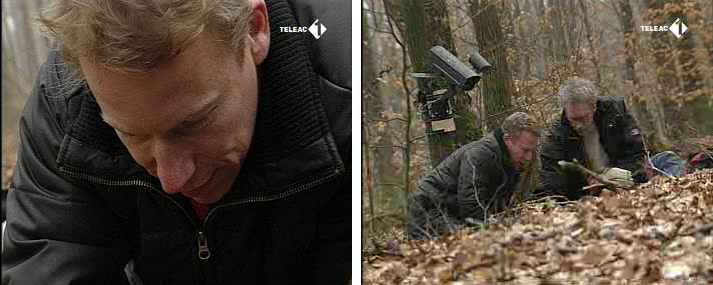
\includegraphics[scale=.5]{images/hard_cut_example.png}
	\caption{These two consecutive frames form a hard cut.}
	\label{fig:hard_cut_example}
\end{figure}

To detect hard cuts, we therefore want to apply a similarity measure to two subsequent frames.
In our case, we represent frames using their color histograms.
Each frame has three color channels (red, green, blue) and therefore three histograms.
The difference between two frames is then the difference between the histograms.
The histogram difference can be represented as a \emph{3*n}-dimensional vector, where \emph{n} is the number of bins in a color histogram.
So, we are presented with a binary classification task (cut or not) in a \emph{3*n}-dimensional space.

In a next step, the dimensionality can be further reduced by simply adding up the vector elements.
This step is justifiable, since it does not matter which color changed and how much, but the sum of changes in all color channels does.
Our results with the reduced dimensionality were better than those of the high dimensional approach.
That's why we use the latter.

To do the actual classification we train an SVM classifier on a labeled training set.
In our implementation, we use the SVM provided by the OpenCV library\footnote{\url{http://docs.opencv.org/doc/tutorials/ml/introduction_to_svm/introduction_to_svm.html}}.
We transform the input space into a higher dimensional feature space by using a kernelized decision function. The commonly used radial basis function (RBF) kernel is employed:
$$K(x_i,x_j) = exp(-\lambda || x_i - x_j ||^2)$$
where $\lambda$ denotes the width of the kernel and $x_i, x_j $ are vectors from the training set.
This is part of the library.
The complexity parameter C for the soft-margin SVM, as well as other parameters are optimized automatically by using the \emph{train\_auto} method of OpenCVs SVM implementation.
It automatically performs a k-fold cross-validation to choose the best parameter values.

\subsection{Visualization}
\label{sec:hard_cut_visualization}

After having implemented the ideas presented in \ref{sec:hard_cut_approach}, the results were not breathtaking. 
Therefore we wanted to get a feel for the flaws in our approach by visualising the features and the decisions that the SVM made.
To make the visualization explorable and interactive, it is a web app written in \emph{HTML} and \emph{Javascript} using \emph{d3}.
During hard cut detection, we write a \emph{tsv} file containing all required information like the histogram differences, the predicted class and the actual class for every two sequent frames.
Then a local webserver is started that has access to the \emph{tsv} file as well as the video frames.
The visualization can then be viewed using a web browser (Figure~\ref{fig:hard_cut_visualization}).

\begin{figure}
	\centering
	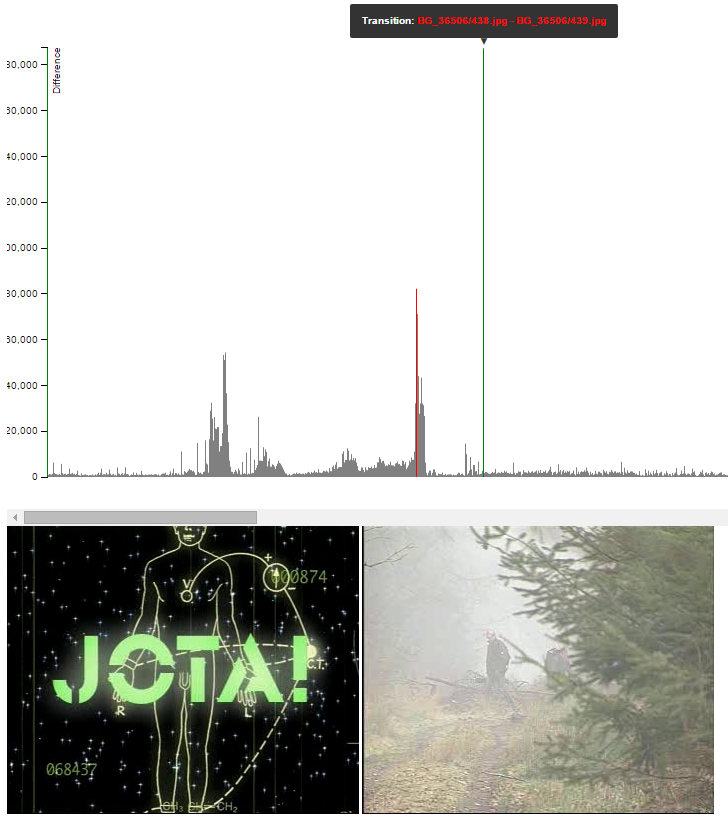
\includegraphics[scale=.7]{images/hard_cut_visualization.png}
	\caption{The height of the bars shows the absolute histogram difference. It is calculated by summing up all elements in the histogram difference vector. The color of the bars indicates the decision: green - true positive, gray - true negative, red - false positive, orange - false negative (not in this picture). When hovering over the bars, the actual frames are shown below together with a tooltip containing the file names.}
	\label{fig:hard_cut_visualization}
\end{figure}


THE FOLLOWING MIGHT BE PART OF THE EVALUATION? \\

When inspecting the visualization of a processed video, we can see that the histogram differences are a useful feature for detecting the hard cuts in a video.
In most cases there is one single bar with a very high difference surrounded by very low differences (see green bar in Figure~\ref{fig:hard_cut_visualization}).
However, we can also see some other peaks that are not hard cuts, which are typically surrounded by noisy clusters (Figure~\ref{fig:hard_cut_noise_visualization}).
Those can be soft cut suquences or just rapid changes during one scene.
Since the SVM just takes the difference between two frames into account, it does not "see" the surrounding clusters and therefore makes several mistakes.

\begin{figure}
	\centering
	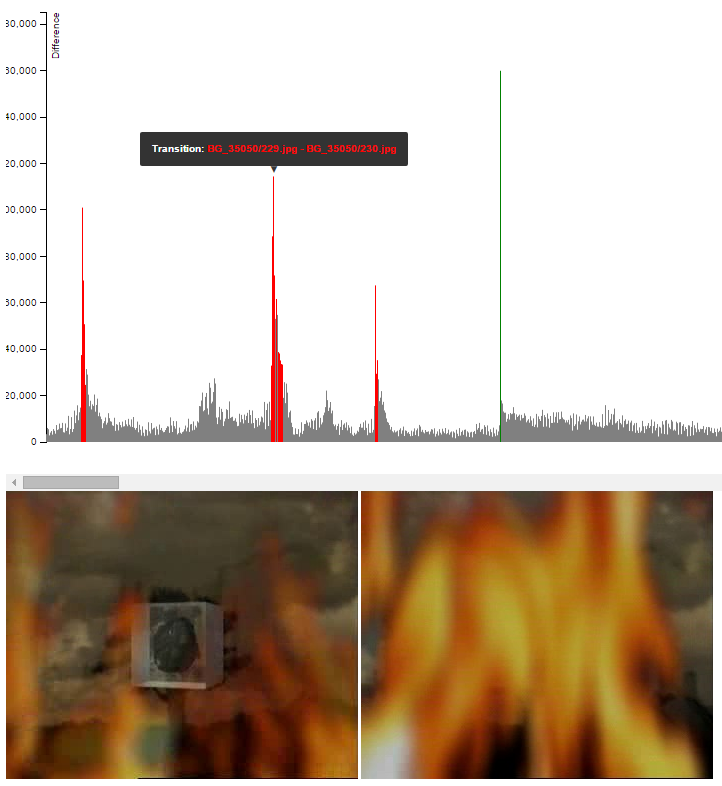
\includegraphics[scale=.7]{images/hard_cut_noise_visualization.png}
	\caption{The histogram differences are problematic when there is lots of noise between two frames. In this case, a burning fire disturbes the classification and introduces lots of false positives.}
	\label{fig:hard_cut_noise_visualization}
\end{figure}
\subsection{Evaluation}
\label{sec:hard_cut_evaluation}

\begin{table}[ht]
	\centering
	\begin{tabular}{l|l}
	Precision & XX \% \\ \hline
	Recall & XX \% \\ \hline
	Accuracy & XX \% \\
	\end{tabular}
	\caption{Results of the hard cut detection}
	\label{tab:hard_cut_results}
\end{table}

\subsubsection{Training Data}
The SVM is trained on an mixture of videos from the 2007 TrecVid contest.
The videos in their full length do not make a good training set, as the ratio between hard cuts and other frames is about \texttt{1:1000}, leading to a failure to predict any hard-cuts.
A custom training set must be constructed, which contains a suffcient amount of hard cuts.
The choice of non-hard-cuts is also crucial for achieving good classification performance: too homogenous frames will lower the decision boundary, and lead to bad performance on noisy examples.
Therefore the negative set should also include soft-cuts and particularly noisy frames.
The training set we finally build consists of about 250 hard cuts and 2200 negatives.


\section{Soft-Cut Detection}
\label{sec:soft_cut}

\subsection{Data Generation}
\label{sec:soft_cut_data_generation}

After having trained a recurrent neural net with the existing data, we noticed that the net did not generalize very well.
In order to solve this problem, more data was necessary.
We decided to generate more data by blending random sequences into each other.
A random sequence is picked by reading the gold standard, picking two consecutive elements which encode two cuts with a start and end frame each.
Between the end frame of the first cut and the start frame of the first cut, we can randomly select a subsequence with the desired transition length (11 and 21).
In order to blend two random sequences, we have multiple options for tweening behaviour.
The standard tweening function is linear, but there are also EaseIn, EaseOut etc. (see Figure~\ref{fig:data_generation}).
The tweening function is randomly selected, as well.

In order to achieve further variance in the generated data, we flip the two sequences randomly at the x- or y-axis or at both axes.
With this approach we generated 50 GB of data.


\begin{figure}
    \centering
    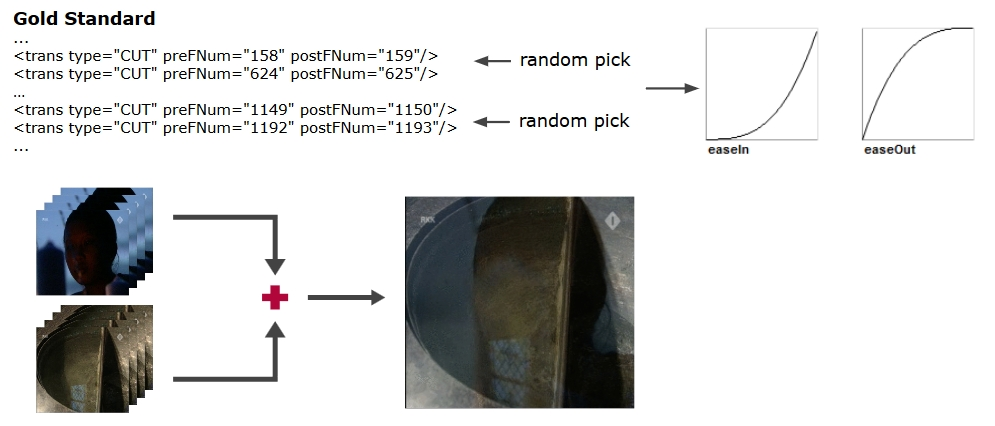
\includegraphics[scale=.5]{images/data_generation.jpg}
    \caption{}
    \label{fig:data_generation}
\end{figure}
\subsection{Approach}
\label{sec:soft_cut_approach}

For the soft cut detection we decided to use a deep learning approach.
More concretely, we used the RNN/LSTM implementation by Jeff Donahue\footnote{\url{https://github.com/BVLC/caffe/pull/2033}} for the Caffe\footnote{\url{http://caffe.berkeleyvision.org/}} framework.
This RNN/LSTM implementation takes two different inputs: On the one hand the raw pixel values and on the other hand a tagging sequence.
The tagging sequence tells the LSTM, where a new training example starts, as we process more than one training sequence per batch.
The LSTM implementation allows us to use a short term memory in the neural network.
The network remembers information from the beginning of a frame sequence until the last frame of the sequence.
So the net remembers previous decisions through a sequence of frames.

But using this architecture has one problem, as stated by Jeff Donahue: ``Backpropagation [through the LSTM] is truncated along the batch boundaries''. % \textcolor{red}{TODO}: Quelle.
So one or more frame sequences have to fit exactly into the batch size used by the RNN/LSTM.
This is hard to achieve, if we want to classify variable-length frame sequences.
Therefore we decided to use a fixed size for the sequences of frames in our training data, i.e. we would generate only transitions of length ten in our training data.

However, we still want to find soft cuts of arbitrary length in a video.
To achieve this, we repeatedly test fixed-size frame sequences.
In Figure~\ref{fig:soft_cut_approach}, we show an example.
\begin{figure}[!htb]
	\centering
	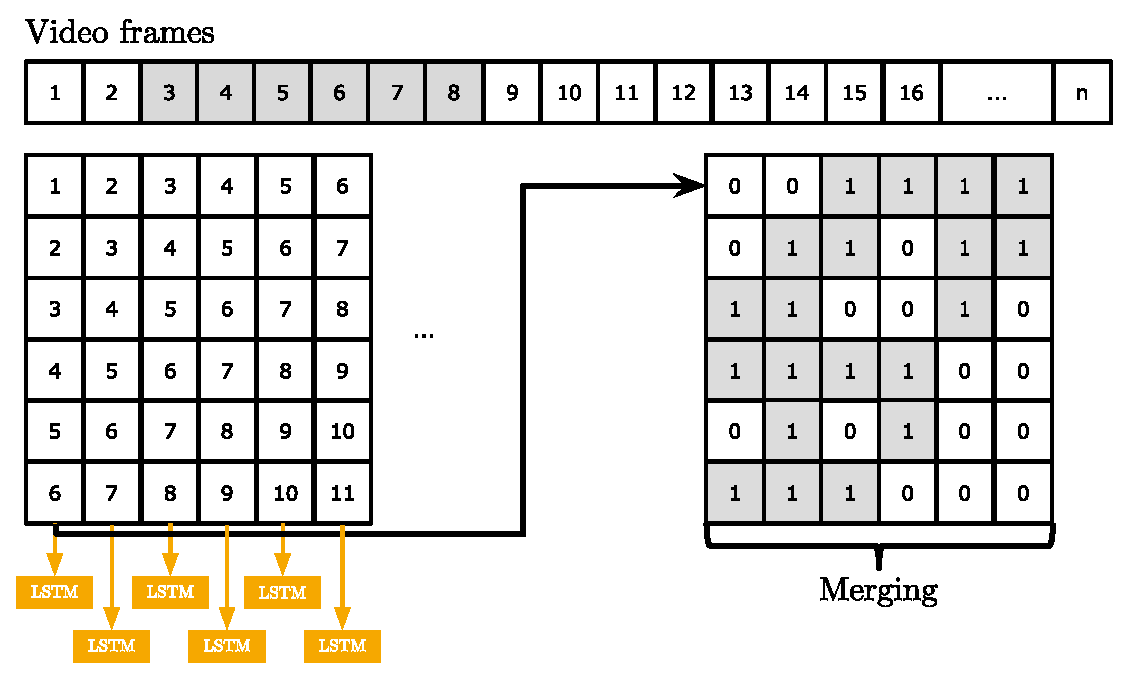
\includegraphics[scale=.7]{images/soft_cut_approach.eps}
	\caption{To classify soft cuts of arbitrary length, we repeatedly test fixed-size frame sequences. In this example we test sequences of size six. Afterwards the predictions given by the RNN/LSTM are merged, so that we have one prediction per frame.}
	\label{fig:soft_cut_approach}
\end{figure}
We have a video with \textit{n} frames.
The frames from three to eight represent a soft cut.
Now, for each frame, we generate a frame sequence of size six starting from that frame.
This is equivalent to moving a sliding window over the frames.
Those sequences are then classified by the RNN/LSTM.
The output of the RNN/LSTM is zero, if a frame does not belong to a soft cut, and one, otherwise.
In the end, we have six predictions per frame, which have to be merged, so that we have only one prediction per frame.
After merging, consecutive frames with a predicted value of 1 represent one soft cut.

In the following several strategies for combining multiple frame predictions into one prediction are presented.
An overview over all strategies can be found in Figure~\ref{fig:merging_strategies}.
\begin{figure}[!htb]
	\centering
	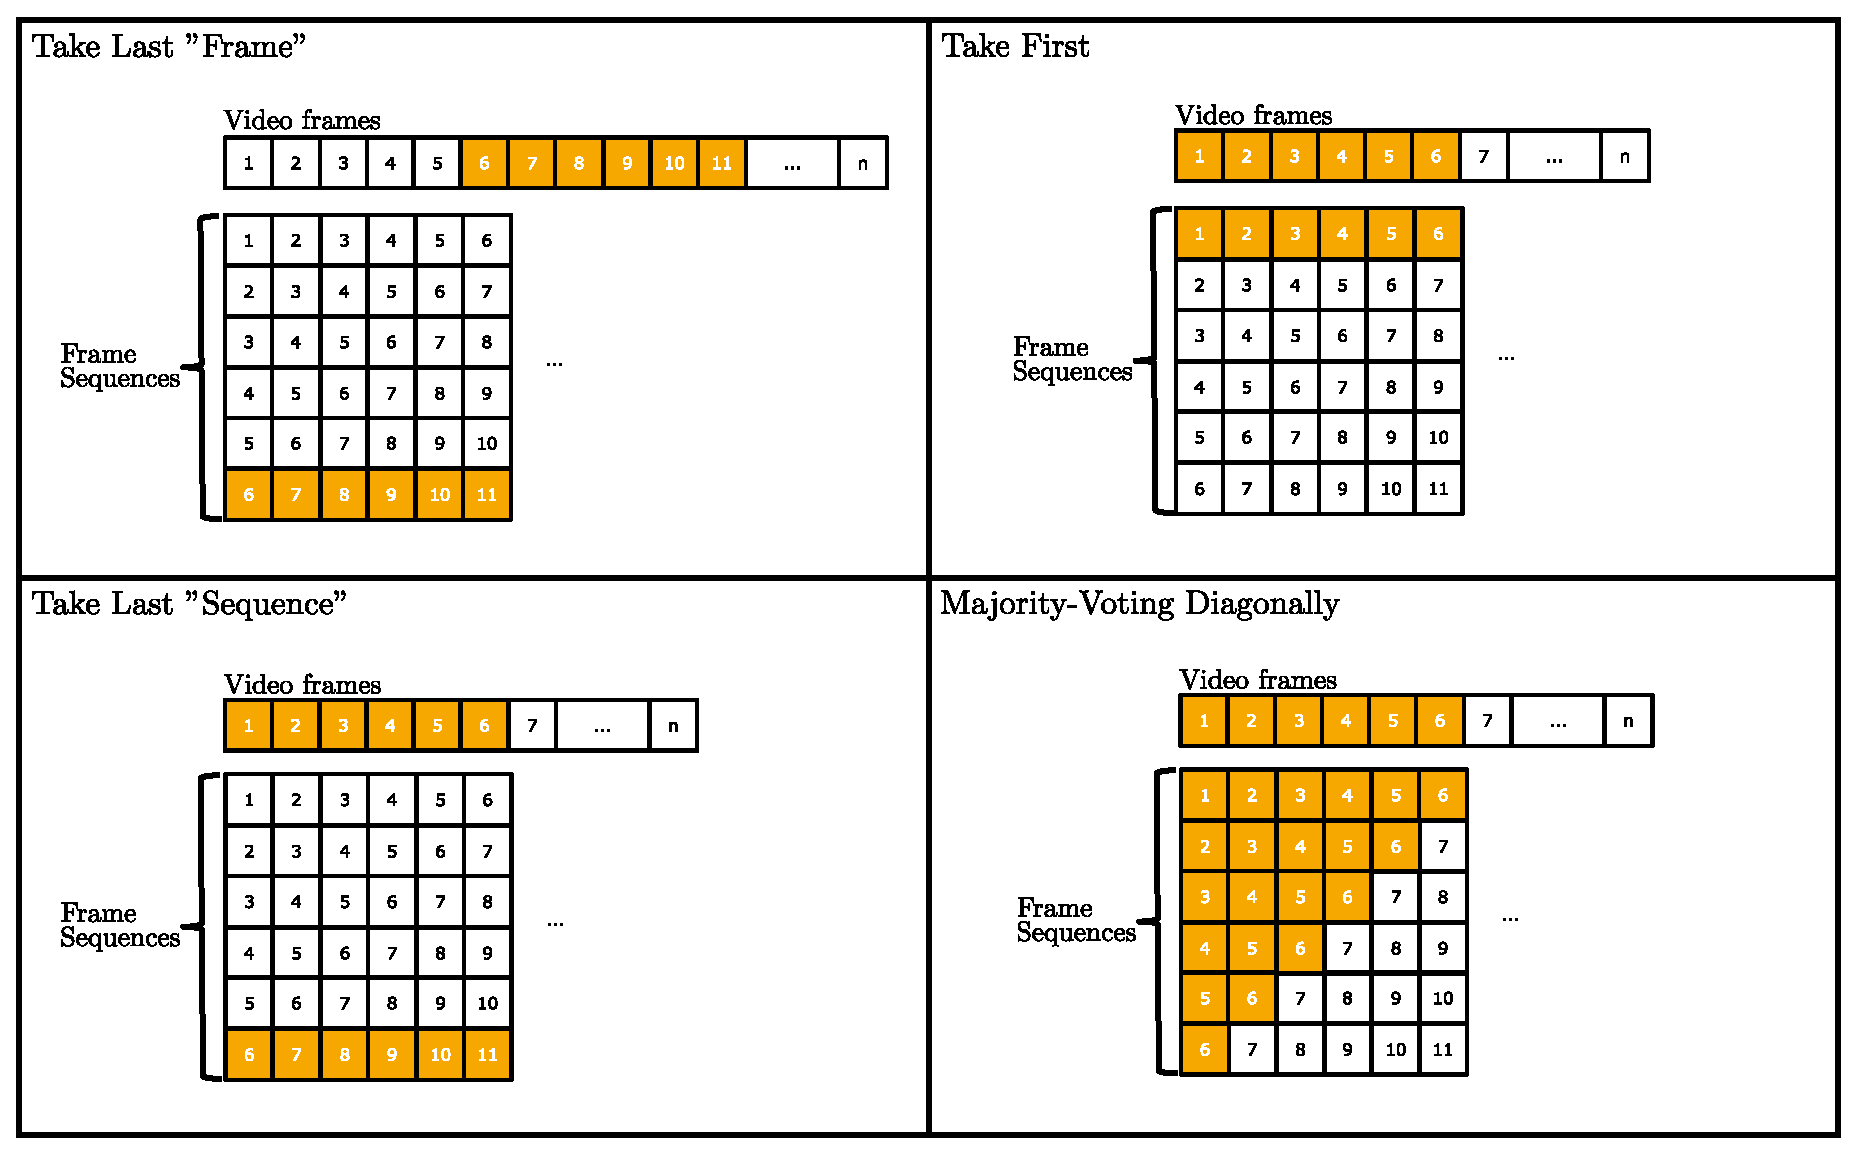
\includegraphics[scale=.5]{images/merging_strategies.eps}
	\caption{To merge the multiple predictions per frame into one, we implemented several strategies:
    \textit{Take Last 'Frame'} (top left): The prediction of the frame, where the frame is the last of a frame sequence, is taken.
    \textit{Take Last 'Sequence'} (bottom left): The last prediction of the frame sequence belonging to a frame is taken.
    \textit{Take First} (top right): The first prediction of the frame sequence is taken.
    \textit{Majority-Voting Diagonally} (bottom right): The majority voting among all predictions of the frame is taken.}
	\label{fig:merging_strategies}
\end{figure}
\paragraph{Take First}
A first simple strategy is to take the first prediction of each sequence as the prediction of that frame.
This is equivalent to having no prior knowledge about the frame, as the RNN/LSTM has not seen any previous frames and therefore could not remember anything.

\paragraph{Take Last 'Sequence'}
A second simple strategy is to take the last prediction of each sequence as the prediction for the frame that started the sequence.
Concretely, the last prediction is not a prediction for the frame under question, but the intuition behind this is that an RNN/LSTM becomes more and more certain after having seen multiple frames of the sequence.

\paragraph{Take Last 'Frame'}
In the \textit{Take Last 'Frame'} strategy, for every frame we take the frame sequence, in which that frame is the last one.
The intuition is similar to the previous case, but now we also use the prediction for the actual frame.

\paragraph{Majority-Voting Diagonally}
Each frame is predicted up to \textit{n} times.
In our example it is up to six times.
In the \textit{Majority-Voting Diagonally} all of those predictions are taken and the majority voting among those is taken as prediction for the frame.
Ties are resolved by placing more weight on the half of the predictions, where the frame appeared later in the sequence.

After merging we have one prediction per frame indicating whether the frame is part of a soft cut or not.
Then, a sequence of frames that are part of a soft cut represents a soft cut.
However, there could be misclassified frame predictions.
We implemented a \textit{Gap Filler} to find and correct some of those misclassified frame predictions.
The \textit{Gap Filler} is looking for sequences of frames that belong to a soft cut and are interrupted by some non cut frames.
If the number of interrupting frames is not too large, they are also classified as soft cut frames.
The idea behind the \textit{Gap Filler} is that two soft cuts do not occur close to each other.
So, if two soft cuts are only a few frames apart, they probably belong to the same soft cut.
In Figure~\ref{fig:gap_filler} an example of the \textit{Gap Filler} is shown.
There, a sequence of soft cut frames is interrupted by two non soft cut frames.
Those non soft cut frames are detected by the \textit{Gap Filler} and classified as soft cut frames.
\begin{figure}[!htb]
	\centering
	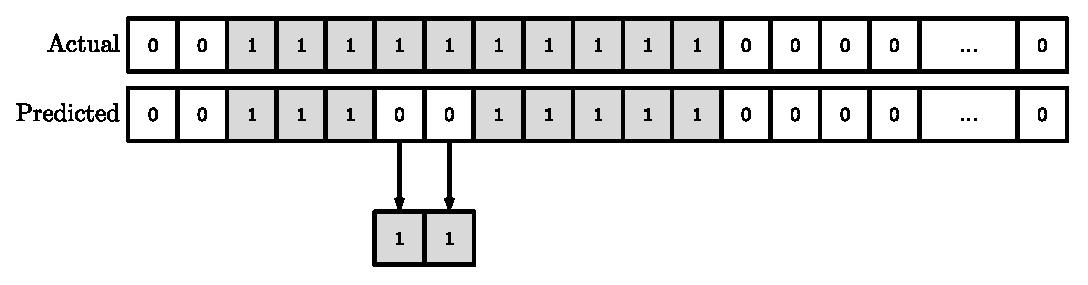
\includegraphics[scale=.7]{images/gap_filler.eps}
	\caption{Two soft cuts do not occur close to each other. Therefore the \textit{Gap Filler} finds misclassified frame predictions after the merging step and corrects non soft cut frame predictions, if they are interrupting a soft cut.}
	\label{fig:gap_filler}
\end{figure}

Another idea for correcting misclassified frame predictions is to delete soft cuts that are only up to five frames long and only surrounded by non soft cut frames.
In our data set a soft cut has an average length of 22 frames.
The smallest have a length of seven frames.
Therefore, a soft cut of only up to five frames is not realistic and misclassified with a high probability.

% \textcolor{red}{TODO}: Ich finde, das sollte doch ein eigener Abschnitt werden, oder?
% Das ist ja jetzt ein komplett anderes Thema auf einmal.
% Und sollte der folgende Teil dann nicht auch zuerst kommen?
% \textcolor{red}{TODO}: Hier muss auch noch hin, we tested many different architectures, and parameters, in the following we present a small selection of that with significant differences.
To classify the frames as soft cut or non soft cut frames, we used an RNN/LSTM.
We tested the following architectures:

\paragraph{CNN + one LSTM}
For the CNN we used the architecture of the \textit{caffenet} [\textcolor{red}{TODO}: reference].
We also used the pre trained weights of this net, so that we do not need to train our model from scratch.
We only fine-tuned the \textit{fc6} layer of the \textit{caffenet} with a learning rate of 0.1.
The CNN is followed by one LSTM, whose weights were initialized with the \textit{Xavier} method [\textcolor{red}{TODO} Zitat: \url{http://jmlr.org/proceedings/papers/v9/glorot10a/glorot10a.pdf}].
Besides, the general learning rate was set to 0.01 and gradient clipping was used.

\paragraph{CNN + two LSTMs}
The architecture of this net is basically the same as the previous.
There is only one difference: Instead of using just one LSTM, two LSTMs were used.
Also the general learning rate was set to 0.001 and no gradient clipping was used.
The architecture of the net can be found in Figure~\ref{fig:net_architecture}.
\begin{figure}[!htb]
	\centering
	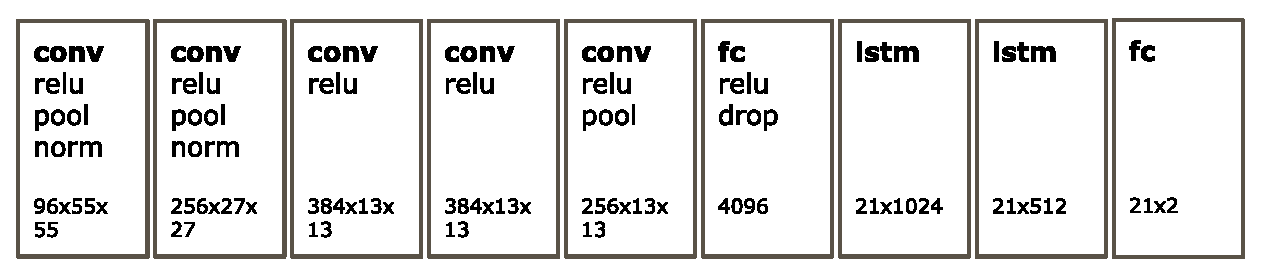
\includegraphics[scale=.5]{images/net_architecture.eps}
	\caption{Architecture of the RNN/LSTM consisting of a CNN and two LSTMs.}
	\label{fig:net_architecture}
\end{figure}

\paragraph{One convolutional layer + two LSTMs}
The last architecture that was tested uses only one convolutional layer before the two LSTMs.
The intuition behind it is as follows: for the CNN, it is hard to detect a soft cut frame, because it works only on one frame.
By looking at only one frame, it would be difficult to predict a soft cut, even for a human.
However, by looking at a sequence of frames, this becomes easier.
This is exactly, what the RNN/LSTM does, which is why we put more emphasis on this part and less emphasis on the CNN part.
The net was trained from scratch as no pretrained net existed.
The weights of the LSTMs were again initialized using the \textit{Xavier} method.
The learning rate was 0.001 and gradient clipping was used during training.


\subsection{Evaluation}
\label{sec:hard_cut_evaluation}

\begin{table}[ht]
	\centering
	\begin{tabular}{l|l}
	Precision & XX \% \\ \hline
	Recall & XX \% \\ \hline
	Accuracy & XX \% \\
	\end{tabular}
	\caption{Results of the hard cut detection}
	\label{tab:hard_cut_results}
\end{table}

\subsubsection{Training Data}
The SVM is trained on an mixture of videos from the 2007 TrecVid contest.
The videos in their full length do not make a good training set, as the ratio between hard cuts and other frames is about \texttt{1:1000}, leading to a failure to predict any hard-cuts.
A custom training set must be constructed, which contains a suffcient amount of hard cuts.
The choice of non-hard-cuts is also crucial for achieving good classification performance: too homogenous frames will lower the decision boundary, and lead to bad performance on noisy examples.
Therefore the negative set should also include soft-cuts and particularly noisy frames.
The training set we finally build consists of about 250 hard cuts and 2200 negatives.


\section{Conclusion}
\label{sec:conclusion}
In the end, we summarize our findings concerning both hard cut and soft cut detection.

\subsection{Hard cut detection}
\label{sec:conclusion_hard_cut}

As we see in Table~\ref{tab:hard_cut_results}, the low precision of our approach is a problem.
We have discussed the main reason for that in Section~\ref{sec:hard_cut_visualization}.
Our approach just takes two frames into account and therefore cannot notice, whether the transition under consideration is part of a noisy cluster or a single peak (see Figure~\ref{fig:hard_cut_noise_visualization}).
One idea to overcome this ``blindness'' is to use some surrounding histogram differences as additional features.
The classifier is trained with a sliding window of histogram differences, resulting in specific patterns.
The classification task would then be a pattern matching task, where hard cuts are characterized by a single peak, soft cuts by a gradual curve, and noise by random peaks.
Future work could also try to employ a neural net for this kind of pattern matching.
A different approach is to do post-processing, where certain highly unlikely events are filtered out.
Looking at the false positives in Figure~\ref{fig:hard_cut_noise_visualization} (red bars), one can see, that many of them occur directly after each other.
Those cut patterns are not realistic.
They might either be noise or a soft cut.

Furthermore, our approach is not applicable for low quality black and white videos (such as the \emph{BG\_11362} video of the TrecVid 2007 data set).
The problem is, that there are strong brightness changes from one frame to another within one scene.
Therefore, we can hardly distinguish between cuts and non-cuts.
An idea to solve this problem is to calculate the brightness difference between the raw pixel values.
If the resulting difference image has homogeneous color, the brightness difference between the two frames is the result of poor image quality.


\subsection{Soft cut detection}
\label{sec:conclusion_hard_cut}

Different from traditional approaches we tried to detect soft cuts in a video using a deep neural network.
As shown in Section~\ref{sec:soft_cut_evaluation} we could only achieve a precision of around 15\% for soft cuts.
We think that there are various reasons for that:
First of all it could still be a lack of insufficient data.
Also the fixed frame sequence length could be a problem.
Training a neural network only with soft cuts of a specific length means that it expected two different frame sequences, which are blend in to each other.
However, in our sliding window approach only a part of a long soft cut is processed at a time.
Maybe the network will not recognize such parts, because the changes are much less and only one of the frame sequences is in the foreground.
This could be evaluated training multiple models each with a different fix sequence length.
For predicting a soft cut of a specific length the corresponding model could be used.

But we think that the main problem is that the convolutional network cannot really learn good features, because there is nothing characteristic about a soft cut frame.
\textcolor{red}{TODO}

In general we still think that the soft cut detection could be solved with deep learning.
However, the basic approach with using a recurrent neural network does not work.
More work and innovation is required in this area.


\bibliography{paper}{}
\bibliographystyle{plain}
\end{document}

